\documentclass[12pt]{article}
\usepackage{tikz}
\usetikzlibrary{bayesnet}
\usepackage{amsmath}
\begin{document}
\section*{Variational Inference for Categorization Notes}
We consider the problem of categorizing stimuli with overlapping distributions
\subsection{Generative model}
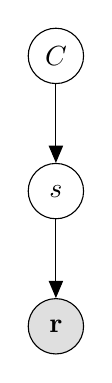
\begin{tikzpicture}
\node[obs]                               (r) {$\mathbf{r}$};
  \node[latent, above=of r] (s) {$s$};
   \node[latent, above=of s]  (c) {$C$};
   \edge {c} {s};
  \edge {s} {r}; 
 \end{tikzpicture}
 \\
$C$ is the category distribution ($\in \{0, 1\}$\\
$P(C) = .5$\\ 
$s$ is the presented stimulus, a draw from the selected category distribution\\
$P(s|C) = \mathcal{N} (s; 0, \sigma_{\text{C}}^2) = \mathcal{N} (s; 0, \tau_{\text{C}}^{-1})$\\
$\mathbf{r}$ is the vector of neural responses to $s$.
$P(r_i|s) = \text{Poisson}(r_i; f_i(s))$\\
~\\
$f_i(s)$ is the tuning curve of the $i^\text{th}$ neuron in response to a stimulus $s$\\
Tuning curve assumptions:
\begin{itemize}
\item Tuning curves cover the space so $\sum_i f_i(s)$ is independent of $s$
\item The tuning curves are Gaussian: $f_i(s) \sim \mathcal{N} (s_i^{\text{pref}}, \sigma_{\text{tc}}^2)$
\end{itemize}

\end{document}